\documentclass[12pt]{article}
\usepackage{latexsym,amssymb,amsmath} % for \Box, \mathbb, split, etc.
% \usepackage[]{showkeys} % shows label names
\usepackage{cite} % sorts citation numbers appropriately
\usepackage{path}
\usepackage{url}
\usepackage{verbatim}
\usepackage[pdftex]{graphicx}
\usepackage{subcaption}
\usepackage{mathtools}

\graphicspath{ {images/} }
% horizontal margins: 1.0 + 6.5 + 1.0 = 8.5
\setlength{\oddsidemargin}{0.0in}
\setlength{\textwidth}{6.5in}
% vertical margins: 1.0 + 9.0 + 1.0 = 11.0
\setlength{\topmargin}{0.0in}
\setlength{\headheight}{12pt}
\setlength{\headsep}{13pt}
\setlength{\textheight}{625pt}
\setlength{\footskip}{24pt}

\renewcommand{\textfraction}{0.10}
\renewcommand{\topfraction}{0.85}
\renewcommand{\bottomfraction}{0.85}
\renewcommand{\floatpagefraction}{0.90}

\makeatletter
\setlength{\arraycolsep}{2\p@} % make spaces around "=" in eqnarray smaller
\makeatother

% change equation, table, figure numbers to be counted inside a section:
\numberwithin{equation}{section}
\numberwithin{table}{section}
\numberwithin{figure}{section}

% begin of personal macros
\newcommand{\half}{{\textstyle \frac{1}{2}}}
\newcommand{\eps}{\varepsilon}
\newcommand{\myth}{\vartheta}
\newcommand{\myphi}{\varphi}

\newcommand{\IN}{\mathbb{N}}
\newcommand{\IZ}{\mathbb{Z}}
\newcommand{\IQ}{\mathbb{Q}}
\newcommand{\IR}{\mathbb{R}}
\newcommand{\IC}{\mathbb{C}}
\newcommand{\Real}[1]{\mathrm{Re}\left({#1}\right)}
\newcommand{\Imag}[1]{\mathrm{Im}\left({#1}\right)}

\newcommand{\norm}[2]{\|{#1}\|_{{}_{#2}}}
\newcommand{\abs}[1]{\left|{#1}\right|}
\newcommand{\ip}[2]{\left\langle {#1}, {#2} \right\rangle}
\newcommand{\der}[2]{\frac{\partial {#1}}{\partial {#2}}}
\newcommand{\dder}[2]{\frac{\partial^2 {#1}}{\partial {#2}^2}}

\newcommand{\nn}{\mathbf{n}}
\newcommand{\xx}{\mathbf{x}}
\newcommand{\uu}{\mathbf{u}}

\newcommand{\junk}[1]{{}}

% set two lengths for the includegraphics commands used to import the plots:
\newlength{\fwtwo} \setlength{\fwtwo}{0.45\textwidth}
% end of personal macros

\begin{document}
%\DeclareGraphicsExtensions{.jpg}

\begin{center}
\textbf{\Large Case Study: Analysis of Shipping Wood to Market} \\[6pt]
  Chetan Gupta \\
  DTU/2K15/CO/044 \\
  Operation Research \\
  MC305 \\[6pt]
  \today
\end{center}

\begin{abstract}
Alabama Atlantic is a lumber company that has three sources of wood and five markets to be supplied. The objective for the OR team is to determine the overall shipping plan that minimizes the total equivalent uniform annual cost. The problem is modelled as a transportation problem and different options are considered to decide on the minimum cost possible.
\end{abstract}

%\subparagraph{Technologies Used.} Python, hd5f, MongoDB, ffmpeg, flask, keras, tensorflow, numpy, charts.js

\section{Introduction}
The Transportation Problem was one of the original applications of linear programming models. It is a special class of linear programs that deals with shipping a commodity from \textit{sources} like factories to \textit{destinations} like warehouses. The objective is to determine the shipping schedule that minimizes the total shipping cost while satisfying supply and demand limits.

\subsection{Short History}

The problem was formalized by the French mathematician Gaspard Monge in 1781. In the 1920s A.N. Tolstoi was one of the first to study the transportation problem mathematically. In 1930, in the collection \textit{Transportation Planning Volume I} for the National Commissariat of Transportation of the Soviet Union, he published a paper \textit{"Methods of Finding the Minimal Kilometrage in Cargo-transportation in space"}. Major advances were made in the field during World War II by the Soviet/Russian mathematician and economist Leonid Kantorovich. Consequently, the problem as it is stated is sometimes known as the \textbf{Monge-Kantorovich transportation problem}.

\subsection{The Transportation Problem Model}
The general transportation problem is considered with distributing \textit{any} commodity from \textit{any} group of supply centers called \textbf{sources}, to \textit{any} group of recieving centers called \textbf{destinations}, in such a way as to minimize the total distribution cost. Each source has a certain \textbf{suppy} and each destination has a certain \textbf{demand}. 

\begin{figure}[h!]
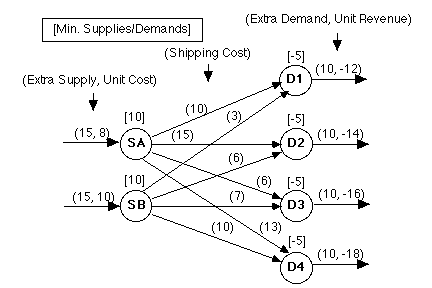
\includegraphics[width = 15cm]{trans_graph}
\centering
\caption{Network Model for Transportation Problem}
\end{figure}

We make the following assumptions :
\begin{itemize}
	\item \textbf{The requirements assumption}\\
		The supply denoted by $s_i$, for \textit{i=1,2,3,...m} and demand denoted by $d_j$, for \textit{j=1,2,3,...n} have fixed values.
	\item \textbf{The feasable solutions property}\\
		The transportaion problem will have feasable solutions if and only if 
		\[ \sum_{i=1}^ms{_i} = \sum_{j=1}^nd{_j} \]
	\item \textbf{The cost assumption}
		The cost of distributing units from any particluar suource to any particular destination is \textit{directly} proportional to the number of units distributed. Therefore the total cost Z :
		\[ \sum_{i=1}^m \sum_{j=1}^nc{_i}{_j}x{_i}{_j} \]
		where $c{_i}{_j}$ is the cost to distribute unit quantity from source i to destination j and $x{_i}{_j}$ is the total quantity distributed from source i to destination j.
\end{itemize}

Thus the linear programming formulation of the problem is :
\begin{equation*}
	\textbf{Minimize} : Z = \sum_{i=1}^m \sum_{j=1}^nc{_i}{_j}x{_i}{_j}
\end{equation*}

\begin{equation*}
	\begin{split}
		\textbf{subject to :} \\
		\sum_{j=1}^nx{_i}{_j} = s{_i}, i=1,2,....m \\
		\sum_{i=1}^mx{_i}{_j} = d{_j}, j=1,2,....n \\
		x{_i}{_j}>=0, \forall i,j
	\end{split}
\end{equation*}

\section{Problem Description}
Alabama Atlantic is a lumber company that has three sources of wood and five markets to be supplied. The annual availability of wood at sources 1, 2, and 3 is 15, 20, and 15 million board feet, respectively. The amount that can be sold annually at markets 1, 2, 3, 4, and 5 is 11, 12, 9, 10, and 8 million board feet, respectively.\\ \\
In the past the company has shipped the wood by train. However, because shipping costs have been increasing, the alternative of using ships to make some of the deliveries is being investigated. This alternative would require the company to invest in some ships. Except for these investment costs, the shipping costs in thousands of dollars per million board feet by rail and by water (when feasible) would be the following for each route: \newpage

\begin{table}[h!]
\centering
\caption{Unit Cost by Rail (\$1,000's)}
\label{railcost}
\begin{tabular}{|c|c|c|c|c|c|}
\hline
\textbf{Source/Dest.} & \textbf{1} & \textbf{2} & \textbf{3} & \textbf{4} & \textbf{5} \\ \hline
\textbf{1}            & 61         & 72         & 45         & 55         & 66         \\ \hline
\textbf{2}            & 69         & 78         & 60         & 49         & 56         \\ \hline
\textbf{3}            & 59         & 66         & 63         & 61         & 47         \\ \hline
\end{tabular}
\end{table}

\begin{table}[h!]
\centering
\caption{Unit Cost by Ship (\$1,000's)}
\label{shipcost}
\begin{tabular}{|c|c|c|c|c|c|}
\hline
\textbf{Source/Dest.} & \textbf{1} & \textbf{2} & \textbf{3} & \textbf{4} & \textbf{5} \\ \hline
\textbf{1}            & 31         & 38         & 24         & -         & 35         \\ \hline
\textbf{2}            & 36         & 43         & 28         & 24         & 31         \\ \hline
\textbf{3}            & -         & 33         & 36         & 32         & 26         \\ \hline
\end{tabular}
\end{table}

The capital investment (in thousands of dollars) in ships required for each million board feet to be transported annually by ship along each route is given as follows:

\begin{table}[h!]
\centering
\caption{Investment for Ships (\$1,000's)}
\label{shipinvest}
\begin{tabular}{|c|c|c|c|c|c|}
\hline
\textbf{Source/Dest.} & \textbf{1} & \textbf{2} & \textbf{3} & \textbf{4} & \textbf{5} \\ \hline
\textbf{1}            & 275         & 303         & 238         & -         & 285         \\ \hline
\textbf{2}            & 293         & 318         & 270         & 250         & 265         \\ \hline
\textbf{3}            & -         & 283         & 275         & 268         & 240        \\ \hline
\end{tabular}
\end{table}

Considering the expected useful life of the ships and the time value of money, the equivalent uniform annual cost of these investments is one-tenth the amount given in the table. The objective is to determine the overall shipping plan that minimizes the total equivalent uniform annual cost (including shipping costs). \\ \\
There are three options for determining the shipping plan :
\begin{enumerate}
	\item Continue shipping exclusively by rail.
	\item Switch to shipping exclusively by water (except where only rail is feasable)
	\item Ship by either rail or water, depending on which is less expensive for the particular route.
\end{enumerate}


\section{Problem Formulation and Calculation}
\subsection{Option 1}
In this option we continue shipping exclusively by rail. We have a parameter table for the unit cost of shipping. We can use the LibreOffice Calc Solver to get the required optimal solution.

\begin{table}[h!]
\centering
\caption{Parameter Table for Rail Only}
\label{param_rail_only}
\begin{tabular}{|c|c|c|c|c|c|}
\hline
\multicolumn{6}{|c|}{\textbf{Unit Cost (\$ 1000's)}}                                                                                                                                                                   \\ \hline
\multicolumn{1}{|l|}{\textbf{Source/Market}} & \multicolumn{1}{l|}{\textbf{1}} & \multicolumn{1}{l|}{\textbf{2}} & \multicolumn{1}{l|}{\textbf{3}} & \multicolumn{1}{l|}{\textbf{4}} & \multicolumn{1}{l|}{\textbf{5}} \\ \hline
\textbf{1}                                   & 61                              & 72                              & 45                              & 55                              & 66                              \\ \hline
\textbf{2}                                   & 69                              & 78                              & 60                              & 49                              & 56                              \\ \hline
\textbf{3}                                   & 59                              & 66                              & 63                              & 61                              & 47                              \\ \hline
\end{tabular}
\end{table}

\begin{table}[h!]
\centering
\caption{Optimal Solution - Only Rail}
\label{optimal_rail}
\begin{tabular}{|c|c|c|c|c|c|c}
\hline
\multicolumn{7}{|c|}{\textbf{Quantity Shipped (mill. board ft)}}                                                                       \\ \hline
\textbf{Source/Market}  & \textbf{1} & \textbf{2} & \textbf{3} & \textbf{4} & \textbf{5} & \multicolumn{1}{c|}{\textbf{Total Shipped}} \\ \hline
\textbf{1}              & 6          & 0          & 9          & 0          & 0          & \multicolumn{1}{c|}{15}                     \\ \hline
\textbf{2}              & 2          & 0          & 0          & 10         & 8          & \multicolumn{1}{c|}{20}                     \\ \hline
\textbf{3}              & 3          & 12         & 9          & 10         & 8          & \multicolumn{1}{c|}{15}                     \\ \hline
\textbf{Total Recieved} & 11         & 12         & 9          & 10         & 8          & \textbf{Total Cost = 2816}                  \\ \cline{1-6}
\end{tabular}
\end{table}

\subsection{Option 2}
In this option we switch to shipping exclusively by water. We have a parameter table for the unit cost of shipping along with required unit cost for investment. The cost for source 1 to market 4 and source 3 to market 1 is kept infinity. We can use the LibreOffice Calc Solver to get the required optimal solution.

\begin{table}[h!]
\centering
\caption{Parameter Table for Ship Only}
\label{param_ship}
\begin{tabular}{|c|c|c|c|c|c|}
\hline
\multicolumn{6}{|c|}{\textbf{Unit Cost (\$1000's)}}                                     \\ \hline
\textbf{Source/Market} & \textbf{1} & \textbf{2} & \textbf{3} & \textbf{4} & \textbf{5} \\ \hline
\textbf{1}             & 58.5       & 68.3       & 47.8       & M          & 63.5       \\ \hline
\textbf{2}             & 65.3       & 74.8       & 55         & 49         & 57.5       \\ \hline
\textbf{3}             & M          & 61.3       & 63.5       & 58.8       & 50         \\ \hline
\end{tabular}
\end{table}

\begin{table}[h!]
\centering
\caption{Optimal Solution - Only Ship}
\label{optimal_ship}
\begin{tabular}{|c|c|c|c|c|c|c}
\hline
\multicolumn{7}{|c|}{\textbf{Quantity Shipped (mill. board ft)}}                                                                       \\ \hline
\textbf{Source/Market}  & \textbf{1} & \textbf{2} & \textbf{3} & \textbf{4} & \textbf{5} & \multicolumn{1}{c|}{\textbf{Total Shipped}} \\ \hline
\textbf{1}              & 6          & 0          & 9          & 0          & 0          & \multicolumn{1}{c|}{15}                     \\ \hline
\textbf{2}              & 5          & 0          & 0          & 10         & 5          & \multicolumn{1}{c|}{20}                     \\ \hline
\textbf{3}              & 0          & 12         & 0          & 0          & 3          & \multicolumn{1}{c|}{15}                     \\ \hline
\textbf{Total Recieved} & 11         & 12         & 9          & 10         & 8          & \textbf{Total Cost = 2770.8}                \\ \cline{1-6}
\end{tabular}
\end{table}



\subsection{Option 3}
In this option we ship either by rail or by water, depending on which is less expensive for the particluar route. We have a parameter table for the unit cost of shipping. We can use the LibreOffice Calc Solver to get the required optimal solution.

\begin{table}[h!]
\centering
\caption{Parameter Table - Min Cost}
\label{param_min}
\begin{tabular}{|c|c|c|c|c|c|}
\hline
\multicolumn{6}{|c|}{\textbf{Unit Cost (\$1000's)}}                                     \\ \hline
\textbf{Source/Market} & \textbf{1} & \textbf{2} & \textbf{3} & \textbf{4} & \textbf{5} \\ \hline
\textbf{1}             & 58.5       & 68.3       & 45         & 55         & 63.5       \\ \hline
\textbf{2}             & 65.3       & 74.8       & 55         & 49         & 56         \\ \hline
\textbf{3}             & 59         & 61.3       & 63         & 58.8       & 47         \\ \hline
\end{tabular}
\end{table}

\begin{table}[h!]
\centering
\caption{Rail or Ship}
\label{ros}
\begin{tabular}{|c|c|c|c|c|c|}
\hline
\multicolumn{6}{|c|}{\textbf{Rail or Ship}}                                             \\ \hline
\textbf{Source/Market} & \textbf{1} & \textbf{2} & \textbf{3} & \textbf{4} & \textbf{5} \\ \hline
\textbf{1}             & S          & S          & R          & R          & R          \\ \hline
\textbf{2}             & S          & S          & S          & R          & R          \\ \hline
\textbf{3}             & R          & S          & R          & S          & R          \\ \hline
\end{tabular}
\end{table}

\begin{table}[h!]
\centering
\caption{Optimal Solution - Minimum Cost}
\label{optimal_min}
\begin{tabular}{|c|c|c|c|c|c|c}
\hline
\multicolumn{7}{|c|}{\textbf{Quantity Shipped (mill. board ft)}}                                                                       \\ \hline
\textbf{Source/Market}  & \textbf{1} & \textbf{2} & \textbf{3} & \textbf{4} & \textbf{5} & \multicolumn{1}{c|}{\textbf{Total Shipped}} \\ \hline
\textbf{1}              & 6          & 0          & 9          & 0          & 0          & \multicolumn{1}{c|}{15}                     \\ \hline
\textbf{2}              & 5          & 0          & 0          & 10         & 5          & \multicolumn{1}{c|}{20}                     \\ \hline
\textbf{3}              & 0          & 12         & 0          & 0          & 3          & \multicolumn{1}{c|}{15}                     \\ \hline
\textbf{Total Recieved} & 11         & 12         & 9          & 10         & 8          & \textbf{Total Cost = 2729.1}                \\ \cline{1-6}
\end{tabular}
\end{table}

\section{Result and Conclusion}
The results from the three options are :
\begin{table}[h!]
\centering
\caption{Total Cost Comparison}
\label{tcc}
\begin{tabular}{|c|c|c|c|}
\hline
\textbf{Option}                & \textbf{1} & \textbf{2} & \textbf{3} \\ \hline
\textbf{Total Cost (\$1000's)} & 2816       & 2770.8     & 2729.1     \\ \hline
\end{tabular}
\end{table}

We can clearly see that changing our distribution network by the use of ships leads to a reduction in total cost by \textbf{\$45,200} anually. Further considering the use of a mixed distribution network,  leads to a further reduction of \textbf{\$41,700} and a total of \textbf{\$86,900}. \\ \\
We conclude by saying that if we invest in new shipping methods while keeping some traditional shipping methods we can achieve more economical costs.

\section{Future Scope}
We can do sensitivity analysis of the model for better forecasting of the future needs. We can also look into using more distribution technologies.

\begin{thebibliography}{3}

\bibitem{stanford_book} 
Frederick S. Hillier \& Gerald J. Lieberman 
\textit{The Transportation and Assignment Problems} “Introduction To Operations Research” 8th edition.
 
\bibitem{Taha} 
Hamdy A. Taha
\textit{The Transportation Model and Its Variant} “Operations Research : An Introduction” 8th edition.

\bibitem{wiki} 
http://wikipedia.com 

\end{thebibliography}



\end{document}